\chapter{Résultats} \label{chap: resultats}

Pour rappeler la chronologie du développement de la méthode, les résultats
présents dans ce chapitre seront décomposés en deux parties~: l'étalonnage et
les plus grands systèmes. Elles expriment respectivement la rigueur attendue
d'une nouvelle implémentation et la réponse à la question~: «\,est-ce que la
méthode demeure pertinente en terrains inconnus\,?\,» c'est-à-dire pour des
systèmes encore jamais résolus avec la CDMFT conventionnelle. Nous commencerons
par valider notre approche sur des systèmes de référence bien connus, en
progressant du plus simple au plus complexe.

\section{Premier étalonnage} \label{sec: etalonnage}

Dans cette section, nous allons reproduire des résultats de CDMFT connus en
séparant le bain en sous-bains en commençant par les systèmes les plus simples
possibles. C'est ce qui nous a permis de tester facilement des hypothèses dans
le développement de la méthode, car certains détails d'implémentation ont
d'abord été choisis empiriquement, comme la pondération uniforme des sous-bains.

Les résultats constitueront toujours une comparaison entre le résultat calculé
en utilisant la CDMFT conventionnelle et celui calculé en morcelant le bain en
plusieurs sous-bains. En utilisant ce format, on compare par exemple le poids
spectral de chaque système en superposant les spectres et appliquant le test
statistique de Kolmogorov-Smirnov~\cite{massey1951kolmogorov} ou encore des
courbes de densité en fonction du potentiel chimique pour mettre l'algorithme au
défi via des dopages hors demi-remplis.

\subsection{Systèmes~1D}

\begin{figure}[h!]
    \centering
    \begin{minipage}{0.48\textwidth}
        \centering
        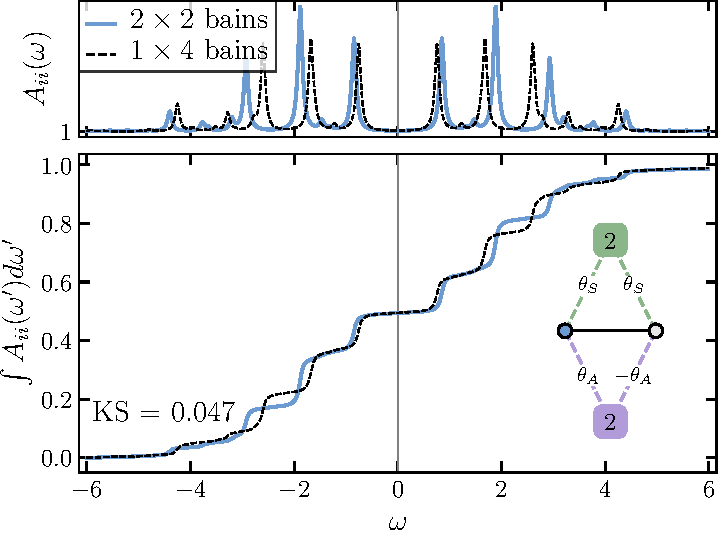
\includegraphics[width=\linewidth]{figs/resultats/2s-4b-1sb_VS_2s-2b-2sb.pdf}
        \caption[Poids spectral d'un système~1x2 avec quatre sites de
        bain.]{\textbf{Poids spectral d'un système~1x2 avec quatre sites de
            bain.} (haut)
         Système de référence à un bain de quatre orbitales de bain en pointillé
         et système séparé en deux sous-bains de deux orbitales de bain en ligne
         pleine. (bas) Sommes cumulatives des poids
         spectraux et test de Kolmogorov-Smirnov (KS) correspondant. Schéma du
         système séparé en sous-bains représentant les secteurs de symétrie
         symétrique $\theta_S$ et antisymétrique $\theta_A$. L'amplitude de
         l'interaction coulombienne est $U/t=4$,
         les sauts sont contraints aux premiers voisins avec une amplitude~$t=1$
     et le potentiel chimique~$\mu=U/2$.}
        \label{fig: 2s-4b-1sb_vs_2s-2b-2sb}
    \end{minipage}
    \hfill
    \begin{minipage}{0.48\textwidth}
        \centering
        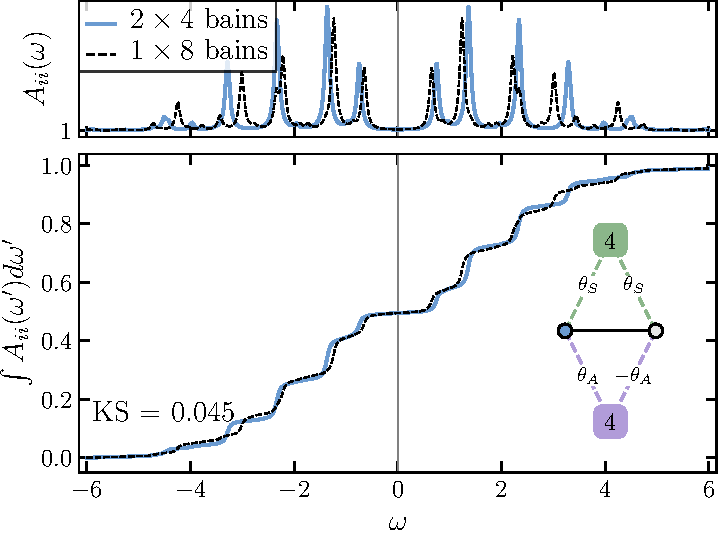
\includegraphics[width=\linewidth]{figs/resultats/2s-8b-1sb_VS_2s-4b-2sb.pdf}
        \caption[Poids spectral d'un système~1x2 avec huit orbitales de
        bain.]{\textbf{Poids spectral d'un système~1x2 avec huit orbitales de
        bain.} Même chose que la figure~\ref{fig: 2s-4b-1sb_vs_2s-2b-2sb}, mais
    le système de référence utilise maintenant un bain de huit orbitales et le
système séparé utilise deux sous-bains de quatre orbitales chacun.}
        \label{fig: 2s-8b-1sb_vs_2s-4b-2sb}
    \end{minipage}
\end{figure}

La figure~\ref{fig: 2s-4b-1sb_vs_2s-2b-2sb} représente le point de départ de
notre validation. Nous avons stratégiquement choisi le plus petit amas possible
(deux sites) avec le plus petit bain pouvant être séparé en sous-bains
significatifs, soit deux sous-bains de deux sites chacun. Le système de
référence correspondant utilise donc un amas de deux sites avec quatre orbitales
de bain. Les fonctions spectrales montrent une correspondance remarquable,
particulièrement à basse fréquence ($\omega\in[-2, 2]$). Cette étonnante
correspondance à basse fréquence s'explique par un aspect subtil de notre
simulation quant à la fréquence de coupure~$i\omega_c=2$ dans la fonction de
distance. L'algorithme de minimisation ajuste donc les paramètres variationnels
pour reproduire fidèlement la physique dans cette fenêtre énergétique.

Aussi, comme démontré dans l'annexe~\ref{chap: ph-symmetry}, la symétrie
particule-trou du modèle d'Anderson à demi-remplissage impose que la fonction
spectrale soit parfaitement symétrique autour de $\omega=0$ lorsque $\mu=U/2$.
Cette propriété est vérifiée dans nos résultats, notamment sur la
figure~\ref{fig: 2s-4b-1sb_vs_2s-2b-2sb}, qui présente une symétrie exacte des
bandes de Hubbard inférieure et supérieure par rapport à $\omega=0$. D'ailleurs,
le gap visible dans les spectres autour de $\omega = 0$ est la signature de
l'isolant de Mott. Physiquement, lorsque $U \gg t$, les électrons se localisent
pour minimiser le coût énergétique de la double occupation. Le système devient
isolant non pas par manque de porteurs de charge (nous comptons un électron par
site), mais parce que le déplacement d’un électron créerait nécessairement une
double occupation coûteuse en énergie. Les deux bandes visibles correspondent
aux excitations de type électron (bande de Hubbard supérieure à $\omega > 0$) et
trou (bande de Hubbard inférieure à $\omega < 0$), séparées par un gap
d'amplitude proportionnelle à $U$.

On note également la présence d'un seul spectre sur la figure~\ref{fig:
2s-4b-1sb_vs_2s-2b-2sb} alors qu'il devrait théoriquement en avoir un pour
chaque site de l'amas~$A_{ii}(\omega)\forall i\in\{1, 2\}$. Toutefois, vu la
symétrie de réflexion~$C_2$ qui s'applique à ces amas, le spectre du site~2 est
identique et donc redondant.

Le système le plus simple étant traité avec succès, il est naturel de vouloir
d'augmenter la taille du système pour vérifier si cet accord tient toujours. Sur
la figure \ref{fig: 2s-8b-1sb_vs_2s-4b-2sb}, nous doublons la taille des bains.
Le système de référence possède huit orbitales de bain, alors que l’algorithme
en sous-bains en possède quatre par sous-bain. L'agrandissement du bain montre
directement une meilleure correspondance entre les fonctions spectrales. En
plus, plus le bain est grand, plus notre gain computationnel l'est aussi. Dans
le cas des résultats de la figure~\ref{fig: 2s-8b-1sb_vs_2s-4b-2sb}, le gain sur
la taille de l'espace de Hilbert à chaque diagonalisation est~:
\begin{align*}
    \frac{4^{N_b(N_{\rm sb}-1)/N_{\rm sb}}}{N_{\rm sb}} = \frac{4^{8(2 -
    1)/2}}{2} = 128.
\end{align*}

\clearpage
